%! Author = trdng
%! Date = 3/2/2026

% Preamble
\documentclass[11pt]{article}

% Packages
\usepackage{braket}
\usepackage{amsmath}
\usepackage{amsfonts}
\usepackage{graphicx}
\usepackage{listings}
\usepackage{xcolor}
\usepackage{indentfirst}


% Listings style
\lstset{
    basicstyle=\ttfamily\small,
    keywordstyle=\color{blue}\bfseries,
    commentstyle=\color{green!50!black}\itshape,
    stringstyle=\color{red},
    showstringspaces=false,
    breaklines=true,
    frame=single
}

% Document
\begin{document}

    \section*{Computational Basis $\{ \ket{0}, \ket{1} \}$}

    $\{\ket{0}, \ket{1}\}$ The set containing the Ket-Zero and Ket-One is the standard set of states used to represent qubits.
    Each qubit can be in superposition of these basis states: $ \ket{\psi} = \alpha \ket{0} + \beta \ket{1} $, where $ \alpha, \beta \in \mathbb{C}$

    \begin{itemize}
        \item When you measure the qubit in the computational basis, the possible outcomes are exactly $ \ket{0} $ and $ \ket{1} $.
        \item The probability of measuring $ \ket{0} $ is $ |\alpha|^2 $, and the probability of measuring $ \ket{1} $ is $ |\beta|^2 $.
    \end{itemize}

    The computation basis defines the \("\)measurement outcomes\("\) are similar to the sample space in classical probability, but the quantum state before measurement is superposition, not a classical probability distribution.
    The probability only emerges upon measurement.

    \begin{figure}[h]  % "h" means "here"
    \centering      % Centers the image
    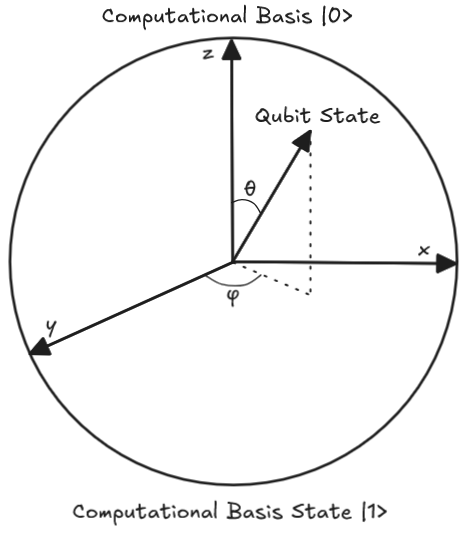
\includegraphics[width=0.6\textwidth]{imgs/Qubit State in Bloch Sphere - Simplified}
    \caption{Qubit in Bloch Sphere}
    \label{fig:qubit_in_bloch_sphere}
    \end{figure}

    \newpage

    \begin{lstlisting}[language=Python, caption={Computational basis declaration},label={lst:lstlisting22}, captionpos=b]
        from qiskit.quantum_info import Statevector

        ket_0 = Statevector.from_label('0')
        ket_1 = Statevector.from_label('1')

        computational_basis = [ket_0, ket_1]
    \end{lstlisting}

\end{document}